% Created by tikzDevice version 0.12.4 on 2023-10-09 16:01:38
% !TEX encoding = UTF-8 Unicode
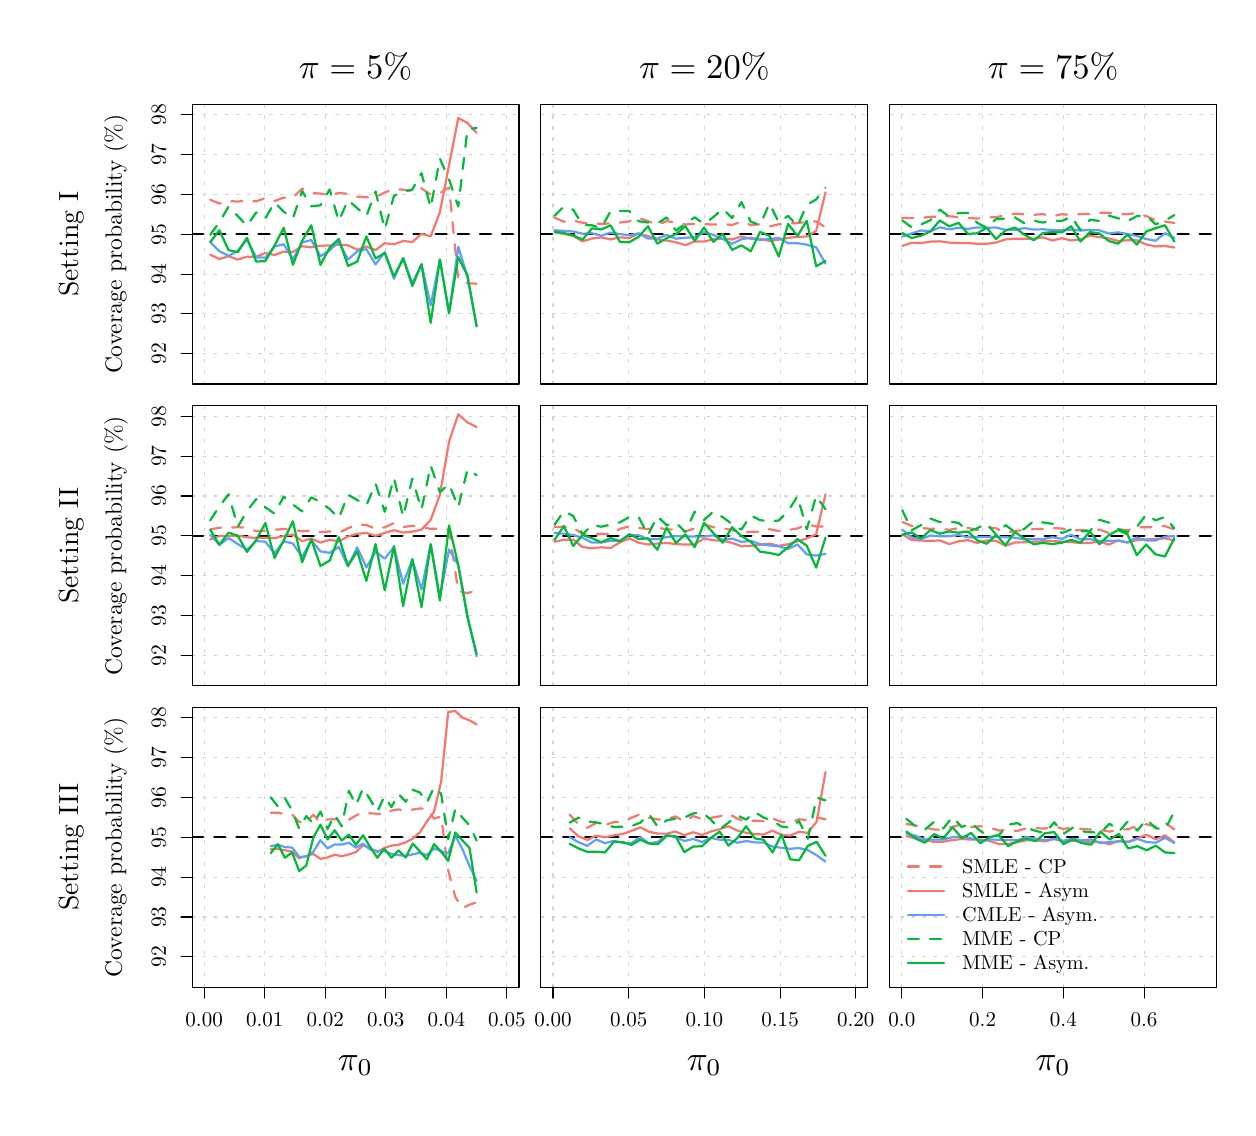
\begin{tikzpicture}[x=1pt,y=1pt]
\definecolor{fillColor}{RGB}{255,255,255}
\path[use as bounding box,fill=fillColor,fill opacity=0.00] (0,0) rectangle (433.62,390.26);
\begin{scope}
\path[clip] ( 55.44,257.53) rectangle (181.50,366.50);
\definecolor{drawColor}{RGB}{0,0,0}

\node[text=drawColor,anchor=base,inner sep=0pt, outer sep=0pt, scale=  0.66] at (118.47,231.40) {Simulation ID};

\node[text=drawColor,rotate= 90.00,anchor=base,inner sep=0pt, outer sep=0pt, scale=  0.66] at ( 34.06,312.01) {Ratio of RMSE};
\end{scope}
\begin{scope}
\path[clip] (  0.00,  0.00) rectangle (433.62,390.26);
\definecolor{drawColor}{RGB}{0,0,0}

\path[draw=drawColor,line width= 0.4pt,line join=round,line cap=round] ( 59.40,272.43) -- ( 59.40,358.80);

\path[draw=drawColor,line width= 0.4pt,line join=round,line cap=round] ( 59.40,272.43) -- ( 55.44,272.43);

\path[draw=drawColor,line width= 0.4pt,line join=round,line cap=round] ( 59.40,286.83) -- ( 55.44,286.83);

\path[draw=drawColor,line width= 0.4pt,line join=round,line cap=round] ( 59.40,301.22) -- ( 55.44,301.22);

\path[draw=drawColor,line width= 0.4pt,line join=round,line cap=round] ( 59.40,315.61) -- ( 55.44,315.61);

\path[draw=drawColor,line width= 0.4pt,line join=round,line cap=round] ( 59.40,330.01) -- ( 55.44,330.01);

\path[draw=drawColor,line width= 0.4pt,line join=round,line cap=round] ( 59.40,344.40) -- ( 55.44,344.40);

\path[draw=drawColor,line width= 0.4pt,line join=round,line cap=round] ( 59.40,358.80) -- ( 55.44,358.80);

\node[text=drawColor,rotate= 90.00,anchor=base,inner sep=0pt, outer sep=0pt, scale=  0.78] at ( 49.90,272.43) {92};

\node[text=drawColor,rotate= 90.00,anchor=base,inner sep=0pt, outer sep=0pt, scale=  0.78] at ( 49.90,286.83) {93};

\node[text=drawColor,rotate= 90.00,anchor=base,inner sep=0pt, outer sep=0pt, scale=  0.78] at ( 49.90,301.22) {94};

\node[text=drawColor,rotate= 90.00,anchor=base,inner sep=0pt, outer sep=0pt, scale=  0.78] at ( 49.90,315.61) {95};

\node[text=drawColor,rotate= 90.00,anchor=base,inner sep=0pt, outer sep=0pt, scale=  0.78] at ( 49.90,330.01) {96};

\node[text=drawColor,rotate= 90.00,anchor=base,inner sep=0pt, outer sep=0pt, scale=  0.78] at ( 49.90,344.40) {97};

\node[text=drawColor,rotate= 90.00,anchor=base,inner sep=0pt, outer sep=0pt, scale=  0.78] at ( 49.90,358.80) {98};
\end{scope}
\begin{scope}
\path[clip] ( 59.40,261.49) rectangle (177.54,362.54);
\definecolor{drawColor}{RGB}{211,211,211}

\path[draw=drawColor,line width= 0.4pt,dash pattern=on 1pt off 3pt ,line join=round,line cap=round] ( 63.78,261.49) -- ( 63.78,362.54);

\path[draw=drawColor,line width= 0.4pt,dash pattern=on 1pt off 3pt ,line join=round,line cap=round] ( 85.65,261.49) -- ( 85.65,362.54);

\path[draw=drawColor,line width= 0.4pt,dash pattern=on 1pt off 3pt ,line join=round,line cap=round] (107.53,261.49) -- (107.53,362.54);

\path[draw=drawColor,line width= 0.4pt,dash pattern=on 1pt off 3pt ,line join=round,line cap=round] (129.41,261.49) -- (129.41,362.54);

\path[draw=drawColor,line width= 0.4pt,dash pattern=on 1pt off 3pt ,line join=round,line cap=round] (151.29,261.49) -- (151.29,362.54);

\path[draw=drawColor,line width= 0.4pt,dash pattern=on 1pt off 3pt ,line join=round,line cap=round] (173.16,261.49) -- (173.16,362.54);

\path[draw=drawColor,line width= 0.4pt,dash pattern=on 1pt off 3pt ,line join=round,line cap=round] ( 59.40,272.43) -- (177.54,272.43);

\path[draw=drawColor,line width= 0.4pt,dash pattern=on 1pt off 3pt ,line join=round,line cap=round] ( 59.40,286.83) -- (177.54,286.83);

\path[draw=drawColor,line width= 0.4pt,dash pattern=on 1pt off 3pt ,line join=round,line cap=round] ( 59.40,301.22) -- (177.54,301.22);

\path[draw=drawColor,line width= 0.4pt,dash pattern=on 1pt off 3pt ,line join=round,line cap=round] ( 59.40,315.61) -- (177.54,315.61);

\path[draw=drawColor,line width= 0.4pt,dash pattern=on 1pt off 3pt ,line join=round,line cap=round] ( 59.40,330.01) -- (177.54,330.01);

\path[draw=drawColor,line width= 0.4pt,dash pattern=on 1pt off 3pt ,line join=round,line cap=round] ( 59.40,344.40) -- (177.54,344.40);

\path[draw=drawColor,line width= 0.4pt,dash pattern=on 1pt off 3pt ,line join=round,line cap=round] ( 59.40,358.80) -- (177.54,358.80);
\end{scope}
\begin{scope}
\path[clip] (  0.00,  0.00) rectangle (433.62,390.26);
\definecolor{drawColor}{RGB}{0,0,0}

\path[draw=drawColor,line width= 0.4pt,line join=round,line cap=round] ( 59.40,261.49) --
	(177.54,261.49) --
	(177.54,362.54) --
	( 59.40,362.54) --
	cycle;
\end{scope}
\begin{scope}
\path[clip] ( 59.40,261.49) rectangle (177.54,362.54);
\definecolor{drawColor}{RGB}{0,0,0}

\path[draw=drawColor,line width= 0.8pt,dash pattern=on 4pt off 4pt ,line join=round,line cap=round] ( 59.40,315.61) -- (177.54,315.61);
\definecolor{drawColor}{RGB}{248,118,109}

\path[draw=drawColor,line width= 0.8pt,dash pattern=on 4pt off 4pt ,line join=round,line cap=round] ( 65.96,328.05) --
	( 69.28,326.70) --
	( 72.60,327.65) --
	( 75.92,327.39) --
	( 79.24,327.88) --
	( 82.56,327.50) --
	( 85.88,328.68) --
	( 89.20,327.62) --
	( 92.52,328.83) --
	( 95.84,328.88) --
	( 99.16,332.08) --
	(102.48,330.53) --
	(105.80,330.30) --
	(109.12,329.83) --
	(112.43,330.53) --
	(115.75,330.21) --
	(119.07,329.20) --
	(122.39,328.97) --
	(125.71,329.00) --
	(129.03,330.70) --
	(132.35,331.94) --
	(135.67,331.71) --
	(138.99,331.19) --
	(142.31,332.17) --
	(145.63,329.95) --
	(148.95,330.47) --
	(152.27,332.51) --
	(155.59,299.38) --
	(158.91,297.88) --
	(162.23,297.74);

\path[draw=drawColor,line width= 0.8pt,line join=round,line cap=round] ( 65.96,308.21) --
	( 69.28,306.66) --
	( 72.60,307.67) --
	( 75.92,306.46) --
	( 79.24,307.52) --
	( 82.56,307.50) --
	( 85.88,308.82) --
	( 89.20,308.10) --
	( 92.52,309.31) --
	( 95.84,309.22) --
	( 99.16,311.27) --
	(102.48,310.89) --
	(105.80,311.47) --
	(109.12,311.55) --
	(112.43,311.78) --
	(115.75,311.61) --
	(119.07,310.03) --
	(122.39,311.18) --
	(125.71,309.91) --
	(129.03,312.36) --
	(132.35,311.99) --
	(135.67,313.19) --
	(138.99,312.80) --
	(142.31,315.74) --
	(145.63,314.86) --
	(148.95,323.55) --
	(152.27,340.66) --
	(155.59,357.59) --
	(158.91,355.83) --
	(162.23,352.26);
\definecolor{drawColor}{RGB}{97,156,255}

\path[draw=drawColor,line width= 0.8pt,line join=round,line cap=round] ( 65.96,312.76) --
	( 69.28,309.48) --
	( 72.60,307.78) --
	( 75.92,309.63) --
	( 79.24,313.71) --
	( 82.56,307.24) --
	( 85.88,307.15) --
	( 89.20,311.18) --
	( 92.52,311.99) --
	( 95.84,306.52) --
	( 99.16,312.65) --
	(102.48,313.51) --
	(105.80,307.67) --
	(109.12,309.80) --
	(112.43,312.91) --
	(115.75,306.43) --
	(119.07,309.40) --
	(122.39,310.23) --
	(125.71,304.70) --
	(129.03,309.11) --
	(132.35,299.52) --
	(135.67,307.03) --
	(138.99,297.85) --
	(142.31,304.76) --
	(145.63,289.96) --
	(148.95,306.40) --
	(152.27,287.20) --
	(155.59,311.06) --
	(158.91,300.33) --
	(162.23,282.36);
\definecolor{drawColor}{RGB}{0,186,56}

\path[draw=drawColor,line width= 0.8pt,dash pattern=on 4pt off 4pt ,line join=round,line cap=round] ( 65.96,315.41) --
	( 69.28,319.96) --
	( 72.60,325.60) --
	( 75.92,322.18) --
	( 79.24,318.64) --
	( 82.56,323.50) --
	( 85.88,321.28) --
	( 89.20,327.13) --
	( 92.52,323.76) --
	( 95.84,321.34) --
	( 99.16,331.22) --
	(102.48,325.69) --
	(105.80,326.06) --
	(109.12,331.79) --
	(112.43,320.36) --
	(115.75,327.99) --
	(119.07,325.03) --
	(122.39,322.18) --
	(125.71,331.04) --
	(129.03,317.48) --
	(132.35,329.46) --
	(135.67,331.02) --
	(138.99,331.76) --
	(142.31,337.67) --
	(145.63,325.20) --
	(148.95,342.96) --
	(152.27,335.39) --
	(155.59,325.66) --
	(158.91,353.47) --
	(162.23,354.02);

\path[draw=drawColor,line width= 0.8pt,line join=round,line cap=round] ( 65.96,312.76) --
	( 69.28,317.02) --
	( 72.60,309.86) --
	( 75.92,309.14) --
	( 79.24,314.32) --
	( 82.56,305.74) --
	( 85.88,305.91) --
	( 89.20,311.50) --
	( 92.52,317.95) --
	( 95.84,304.56) --
	( 99.16,313.22) --
	(102.48,318.84) --
	(105.80,304.53) --
	(109.12,310.75) --
	(112.43,313.92) --
	(115.75,304.16) --
	(119.07,305.71) --
	(122.39,314.84) --
	(125.71,306.86) --
	(129.03,308.85) --
	(132.35,300.36) --
	(135.67,306.89) --
	(138.99,296.93) --
	(142.31,304.79) --
	(145.63,283.60) --
	(148.95,306.52) --
	(152.27,287.06) --
	(155.59,307.38) --
	(158.91,300.70) --
	(162.23,282.33);
\end{scope}
\begin{scope}
\path[clip] (  0.00,  0.00) rectangle (433.62,390.26);
\definecolor{drawColor}{RGB}{0,0,0}

\node[text=drawColor,rotate= 90.00,anchor=base,inner sep=0pt, outer sep=0pt, scale=  1.00] at ( 18.22,312.01) {Setting I};

\node[text=drawColor,rotate= 90.00,anchor=base,inner sep=0pt, outer sep=0pt, scale=  0.85] at ( 34.06,312.01) {Coverage probability ($\%$)};

\node[text=drawColor,anchor=base,inner sep=0pt, outer sep=0pt, scale=  1.25] at (118.47,372.04) {$\pi = 5\%$};
\end{scope}
\begin{scope}
\path[clip] (181.50,257.53) rectangle (307.56,366.50);
\definecolor{drawColor}{RGB}{0,0,0}

\node[text=drawColor,anchor=base,inner sep=0pt, outer sep=0pt, scale=  0.66] at (244.53,231.40) {Simulation ID};

\node[text=drawColor,rotate= 90.00,anchor=base,inner sep=0pt, outer sep=0pt, scale=  0.66] at (160.12,312.01) {Ratio of RMSE};
\end{scope}
\begin{scope}
\path[clip] (185.46,261.49) rectangle (303.60,362.54);
\definecolor{drawColor}{RGB}{211,211,211}

\path[draw=drawColor,line width= 0.4pt,dash pattern=on 1pt off 3pt ,line join=round,line cap=round] (189.84,261.49) -- (189.84,362.54);

\path[draw=drawColor,line width= 0.4pt,dash pattern=on 1pt off 3pt ,line join=round,line cap=round] (217.18,261.49) -- (217.18,362.54);

\path[draw=drawColor,line width= 0.4pt,dash pattern=on 1pt off 3pt ,line join=round,line cap=round] (244.53,261.49) -- (244.53,362.54);

\path[draw=drawColor,line width= 0.4pt,dash pattern=on 1pt off 3pt ,line join=round,line cap=round] (271.88,261.49) -- (271.88,362.54);

\path[draw=drawColor,line width= 0.4pt,dash pattern=on 1pt off 3pt ,line join=round,line cap=round] (299.22,261.49) -- (299.22,362.54);

\path[draw=drawColor,line width= 0.4pt,dash pattern=on 1pt off 3pt ,line join=round,line cap=round] (185.46,272.43) -- (303.60,272.43);

\path[draw=drawColor,line width= 0.4pt,dash pattern=on 1pt off 3pt ,line join=round,line cap=round] (185.46,286.83) -- (303.60,286.83);

\path[draw=drawColor,line width= 0.4pt,dash pattern=on 1pt off 3pt ,line join=round,line cap=round] (185.46,301.22) -- (303.60,301.22);

\path[draw=drawColor,line width= 0.4pt,dash pattern=on 1pt off 3pt ,line join=round,line cap=round] (185.46,315.61) -- (303.60,315.61);

\path[draw=drawColor,line width= 0.4pt,dash pattern=on 1pt off 3pt ,line join=round,line cap=round] (185.46,330.01) -- (303.60,330.01);

\path[draw=drawColor,line width= 0.4pt,dash pattern=on 1pt off 3pt ,line join=round,line cap=round] (185.46,344.40) -- (303.60,344.40);

\path[draw=drawColor,line width= 0.4pt,dash pattern=on 1pt off 3pt ,line join=round,line cap=round] (185.46,358.80) -- (303.60,358.80);
\end{scope}
\begin{scope}
\path[clip] (  0.00,  0.00) rectangle (433.62,390.26);
\definecolor{drawColor}{RGB}{0,0,0}

\path[draw=drawColor,line width= 0.4pt,line join=round,line cap=round] (185.46,261.49) --
	(303.60,261.49) --
	(303.60,362.54) --
	(185.46,362.54) --
	cycle;
\end{scope}
\begin{scope}
\path[clip] (185.46,261.49) rectangle (303.60,362.54);
\definecolor{drawColor}{RGB}{0,0,0}

\path[draw=drawColor,line width= 0.8pt,dash pattern=on 4pt off 4pt ,line join=round,line cap=round] (185.46,315.61) -- (303.60,315.61);
\definecolor{drawColor}{RGB}{248,118,109}

\path[draw=drawColor,line width= 0.8pt,line join=round,line cap=round] (190.38,316.33) --
	(193.76,315.73) --
	(197.13,315.01) --
	(200.51,313.05) --
	(203.89,314.06) --
	(207.26,314.49) --
	(210.64,313.74) --
	(214.01,314.49) --
	(217.39,314.26) --
	(220.77,315.84) --
	(224.14,314.98) --
	(227.52,313.71) --
	(230.89,313.34) --
	(234.27,312.71) --
	(237.65,311.67) --
	(241.02,312.99) --
	(244.40,312.97) --
	(247.77,313.77) --
	(251.15,314.06) --
	(254.53,313.71) --
	(257.90,314.84) --
	(261.28,313.94) --
	(264.65,314.03) --
	(268.03,313.17) --
	(271.41,313.66) --
	(274.78,314.29) --
	(278.16,314.69) --
	(281.53,314.77) --
	(284.91,316.83) --
	(288.29,330.71);

\path[draw=drawColor,line width= 0.8pt,dash pattern=on 4pt off 4pt ,line join=round,line cap=round] (190.38,321.60) --
	(193.76,320.16) --
	(197.13,320.57) --
	(200.51,319.76) --
	(203.89,319.53) --
	(207.26,319.36) --
	(210.64,319.53) --
	(214.01,319.82) --
	(217.39,320.25) --
	(220.77,321.49) --
	(224.14,320.36) --
	(227.52,318.95) --
	(230.89,320.33) --
	(234.27,319.85) --
	(237.65,319.15) --
	(241.02,319.36) --
	(244.40,319.27) --
	(247.77,319.10) --
	(251.15,319.33) --
	(254.53,318.95) --
	(257.90,320.19) --
	(261.28,318.95) --
	(264.65,319.21) --
	(268.03,318.41) --
	(271.41,319.21) --
	(274.78,319.47) --
	(278.16,319.67) --
	(281.53,320.08) --
	(284.91,320.25) --
	(288.29,318.15);
\definecolor{drawColor}{RGB}{97,156,255}

\path[draw=drawColor,line width= 0.8pt,line join=round,line cap=round] (190.38,317.05) --
	(193.76,316.85) --
	(197.13,316.59) --
	(200.51,315.79) --
	(203.89,315.99) --
	(207.26,315.07) --
	(210.64,316.22) --
	(214.01,315.67) --
	(217.39,315.24) --
	(220.77,315.93) --
	(224.14,314.09) --
	(227.52,314.03) --
	(230.89,315.38) --
	(234.27,314.00) --
	(237.65,314.35) --
	(241.02,314.55) --
	(244.40,316.36) --
	(247.77,315.38) --
	(251.15,313.92) --
	(254.53,312.16) --
	(257.90,313.80) --
	(261.28,314.40) --
	(264.65,313.54) --
	(268.03,313.92) --
	(271.41,314.29) --
	(274.78,312.36) --
	(278.16,312.36) --
	(281.53,311.84) --
	(284.91,310.89) --
	(288.29,304.99);
\definecolor{drawColor}{RGB}{0,186,56}

\path[draw=drawColor,line width= 0.8pt,dash pattern=on 4pt off 4pt ,line join=round,line cap=round] (190.38,322.23) --
	(193.76,325.66) --
	(197.13,324.45) --
	(200.51,318.98) --
	(203.89,318.84) --
	(207.26,317.86) --
	(210.64,323.93) --
	(214.01,323.99) --
	(217.39,323.99) --
	(220.77,320.31) --
	(224.14,319.85) --
	(227.52,319.50) --
	(230.89,321.69) --
	(234.27,316.94) --
	(237.65,319.50) --
	(241.02,321.72) --
	(244.40,319.33) --
	(247.77,321.80) --
	(251.15,324.88) --
	(254.53,321.46) --
	(257.90,327.22) --
	(261.28,320.10) --
	(264.65,318.98) --
	(268.03,326.75) --
	(271.41,319.96) --
	(274.78,322.26) --
	(278.16,318.55) --
	(281.53,326.27) --
	(284.91,328.17) --
	(288.29,332.45);

\path[draw=drawColor,line width= 0.8pt,line join=round,line cap=round] (190.38,316.51) --
	(193.76,316.05) --
	(197.13,315.21) --
	(200.51,313.66) --
	(203.89,317.74) --
	(207.26,317.34) --
	(210.64,318.84) --
	(214.01,312.85) --
	(217.39,312.71) --
	(220.77,314.72) --
	(224.14,318.49) --
	(227.52,312.22) --
	(230.89,314.20) --
	(234.27,315.64) --
	(237.65,318.52) --
	(241.02,313.20) --
	(244.40,318.03) --
	(247.77,312.88) --
	(251.15,315.73) --
	(254.53,309.94) --
	(257.90,311.61) --
	(261.28,309.45) --
	(264.65,316.48) --
	(268.03,315.01) --
	(271.41,307.55) --
	(274.78,319.33) --
	(278.16,315.01) --
	(281.53,320.48) --
	(284.91,304.04) --
	(288.29,305.97);
\end{scope}
\begin{scope}
\path[clip] (  0.00,  0.00) rectangle (433.62,390.26);
\definecolor{drawColor}{RGB}{0,0,0}

\node[text=drawColor,anchor=base,inner sep=0pt, outer sep=0pt, scale=  1.25] at (244.53,372.04) {$\pi= 20\%$};
\end{scope}
\begin{scope}
\path[clip] (307.56,257.53) rectangle (433.62,366.50);
\definecolor{drawColor}{RGB}{0,0,0}

\node[text=drawColor,anchor=base,inner sep=0pt, outer sep=0pt, scale=  0.66] at (370.59,231.40) {Simulation ID};

\node[text=drawColor,rotate= 90.00,anchor=base,inner sep=0pt, outer sep=0pt, scale=  0.66] at (286.18,312.01) {Ratio of RMSE};
\end{scope}
\begin{scope}
\path[clip] (311.52,261.49) rectangle (429.66,362.54);
\definecolor{drawColor}{RGB}{211,211,211}

\path[draw=drawColor,line width= 0.4pt,dash pattern=on 1pt off 3pt ,line join=round,line cap=round] (315.90,261.49) -- (315.90,362.54);

\path[draw=drawColor,line width= 0.4pt,dash pattern=on 1pt off 3pt ,line join=round,line cap=round] (345.07,261.49) -- (345.07,362.54);

\path[draw=drawColor,line width= 0.4pt,dash pattern=on 1pt off 3pt ,line join=round,line cap=round] (374.24,261.49) -- (374.24,362.54);

\path[draw=drawColor,line width= 0.4pt,dash pattern=on 1pt off 3pt ,line join=round,line cap=round] (403.41,261.49) -- (403.41,362.54);

\path[draw=drawColor,line width= 0.4pt,dash pattern=on 1pt off 3pt ,line join=round,line cap=round] (311.52,272.43) -- (429.66,272.43);

\path[draw=drawColor,line width= 0.4pt,dash pattern=on 1pt off 3pt ,line join=round,line cap=round] (311.52,286.83) -- (429.66,286.83);

\path[draw=drawColor,line width= 0.4pt,dash pattern=on 1pt off 3pt ,line join=round,line cap=round] (311.52,301.22) -- (429.66,301.22);

\path[draw=drawColor,line width= 0.4pt,dash pattern=on 1pt off 3pt ,line join=round,line cap=round] (311.52,315.61) -- (429.66,315.61);

\path[draw=drawColor,line width= 0.4pt,dash pattern=on 1pt off 3pt ,line join=round,line cap=round] (311.52,330.01) -- (429.66,330.01);

\path[draw=drawColor,line width= 0.4pt,dash pattern=on 1pt off 3pt ,line join=round,line cap=round] (311.52,344.40) -- (429.66,344.40);

\path[draw=drawColor,line width= 0.4pt,dash pattern=on 1pt off 3pt ,line join=round,line cap=round] (311.52,358.80) -- (429.66,358.80);
\end{scope}
\begin{scope}
\path[clip] (  0.00,  0.00) rectangle (433.62,390.26);
\definecolor{drawColor}{RGB}{0,0,0}

\path[draw=drawColor,line width= 0.4pt,line join=round,line cap=round] (311.52,261.49) --
	(429.66,261.49) --
	(429.66,362.54) --
	(311.52,362.54) --
	cycle;
\end{scope}
\begin{scope}
\path[clip] (311.52,261.49) rectangle (429.66,362.54);
\definecolor{drawColor}{RGB}{0,0,0}

\path[draw=drawColor,line width= 0.8pt,dash pattern=on 4pt off 4pt ,line join=round,line cap=round] (311.52,315.61) -- (429.66,315.61);
\definecolor{drawColor}{RGB}{248,118,109}

\path[draw=drawColor,line width= 0.8pt,dash pattern=on 4pt off 4pt ,line join=round,line cap=round] (316.04,321.43) --
	(319.43,321.52) --
	(322.82,321.52) --
	(326.21,321.89) --
	(329.60,321.92) --
	(332.99,322.12) --
	(336.38,321.77) --
	(339.77,321.54) --
	(343.16,321.26) --
	(346.55,321.72) --
	(349.94,321.77) --
	(353.33,322.49) --
	(356.72,323.04) --
	(360.11,322.81) --
	(363.50,322.64) --
	(366.89,322.87) --
	(370.28,322.09) --
	(373.67,322.84) --
	(377.06,322.61) --
	(380.45,322.87) --
	(383.84,322.95) --
	(387.23,323.36) --
	(390.62,323.39) --
	(394.01,322.70) --
	(397.40,322.90) --
	(400.79,323.21) --
	(404.18,322.15) --
	(407.57,320.71) --
	(410.96,320.22) --
	(414.35,319.70);

\path[draw=drawColor,line width= 0.8pt,line join=round,line cap=round] (316.04,311.41) --
	(319.43,312.53) --
	(322.82,312.42) --
	(326.21,312.94) --
	(329.60,313.05) --
	(332.99,312.59) --
	(336.38,312.45) --
	(339.77,312.42) --
	(343.16,312.16) --
	(346.55,312.16) --
	(349.94,312.62) --
	(353.33,313.74) --
	(356.72,313.97) --
	(360.11,314.00) --
	(363.50,313.94) --
	(366.89,314.49) --
	(370.28,313.34) --
	(373.67,314.17) --
	(377.06,313.37) --
	(380.45,313.74) --
	(383.84,315.18) --
	(387.23,314.55) --
	(390.62,314.12) --
	(394.01,313.17) --
	(397.40,313.43) --
	(400.79,313.43) --
	(404.18,311.93) --
	(407.57,311.21) --
	(410.96,311.35) --
	(414.35,310.83);
\definecolor{drawColor}{RGB}{97,156,255}

\path[draw=drawColor,line width= 0.8pt,line join=round,line cap=round] (316.04,314.75) --
	(319.43,315.93) --
	(322.82,316.97) --
	(326.21,316.68) --
	(329.60,318.12) --
	(332.99,317.37) --
	(336.38,317.95) --
	(339.77,317.54) --
	(343.16,318.09) --
	(346.55,317.97) --
	(349.94,318.03) --
	(353.33,317.20) --
	(356.72,317.17) --
	(360.11,317.83) --
	(363.50,317.31) --
	(366.89,317.40) --
	(370.28,317.14) --
	(373.67,317.05) --
	(377.06,317.28) --
	(380.45,316.94) --
	(383.84,317.23) --
	(387.23,317.05) --
	(390.62,315.87) --
	(394.01,316.30) --
	(397.40,315.70) --
	(400.79,314.98) --
	(404.18,313.89) --
	(407.57,313.28) --
	(410.96,315.99) --
	(414.35,314.26);
\definecolor{drawColor}{RGB}{0,186,56}

\path[draw=drawColor,line width= 0.8pt,dash pattern=on 4pt off 4pt ,line join=round,line cap=round] (316.04,320.62) --
	(319.43,318.12) --
	(322.82,319.13) --
	(326.21,320.71) --
	(329.60,324.51) --
	(332.99,321.95) --
	(336.38,323.27) --
	(339.77,323.27) --
	(343.16,319.70) --
	(346.55,317.97) --
	(349.94,321.08) --
	(353.33,321.26) --
	(356.72,321.72) --
	(360.11,319.59) --
	(363.50,320.51) --
	(366.89,319.82) --
	(370.28,320.57) --
	(373.67,320.36) --
	(377.06,322.03) --
	(380.45,317.08) --
	(383.84,320.85) --
	(387.23,320.42) --
	(390.62,322.35) --
	(394.01,321.40) --
	(397.40,320.33) --
	(400.79,322.15) --
	(404.18,322.38) --
	(407.57,319.21) --
	(410.96,320.48) --
	(414.35,322.55);

\path[draw=drawColor,line width= 0.8pt,line join=round,line cap=round] (316.04,316.05) --
	(319.43,314.26) --
	(322.82,315.10) --
	(326.21,316.65) --
	(329.60,320.57) --
	(332.99,318.49) --
	(336.38,319.73) --
	(339.77,315.73) --
	(343.16,315.96) --
	(346.55,317.97) --
	(349.94,313.89) --
	(353.33,316.97) --
	(356.72,318.03) --
	(360.11,315.50) --
	(363.50,313.43) --
	(366.89,316.07) --
	(370.28,316.39) --
	(373.67,316.28) --
	(377.06,318.49) --
	(380.45,312.94) --
	(383.84,316.39) --
	(387.23,315.90) --
	(390.62,313.17) --
	(394.01,312.19) --
	(397.40,315.50) --
	(400.79,311.87) --
	(404.18,316.62) --
	(407.57,317.80) --
	(410.96,318.87) --
	(414.35,312.97);
\end{scope}
\begin{scope}
\path[clip] (  0.00,  0.00) rectangle (433.62,390.26);
\definecolor{drawColor}{RGB}{0,0,0}

\node[text=drawColor,anchor=base,inner sep=0pt, outer sep=0pt, scale=  1.25] at (370.59,372.04) {$\pi= 75\%$};
\end{scope}
\begin{scope}
\path[clip] ( 55.44,148.57) rectangle (181.50,257.53);
\definecolor{drawColor}{RGB}{0,0,0}

\node[text=drawColor,anchor=base,inner sep=0pt, outer sep=0pt, scale=  0.66] at (118.47,122.43) {Simulation ID};

\node[text=drawColor,rotate= 90.00,anchor=base,inner sep=0pt, outer sep=0pt, scale=  0.66] at ( 34.06,203.05) {Ratio of RMSE};
\end{scope}
\begin{scope}
\path[clip] ( 59.40,152.53) rectangle (177.54,253.57);
\definecolor{drawColor}{RGB}{211,211,211}

\path[draw=drawColor,line width= 0.4pt,dash pattern=on 1pt off 3pt ,line join=round,line cap=round] ( 63.78,152.53) -- ( 63.78,253.57);

\path[draw=drawColor,line width= 0.4pt,dash pattern=on 1pt off 3pt ,line join=round,line cap=round] ( 85.65,152.53) -- ( 85.65,253.57);

\path[draw=drawColor,line width= 0.4pt,dash pattern=on 1pt off 3pt ,line join=round,line cap=round] (107.53,152.53) -- (107.53,253.57);

\path[draw=drawColor,line width= 0.4pt,dash pattern=on 1pt off 3pt ,line join=round,line cap=round] (129.41,152.53) -- (129.41,253.57);

\path[draw=drawColor,line width= 0.4pt,dash pattern=on 1pt off 3pt ,line join=round,line cap=round] (151.29,152.53) -- (151.29,253.57);

\path[draw=drawColor,line width= 0.4pt,dash pattern=on 1pt off 3pt ,line join=round,line cap=round] (173.16,152.53) -- (173.16,253.57);

\path[draw=drawColor,line width= 0.4pt,dash pattern=on 1pt off 3pt ,line join=round,line cap=round] ( 59.40,163.47) -- (177.54,163.47);

\path[draw=drawColor,line width= 0.4pt,dash pattern=on 1pt off 3pt ,line join=round,line cap=round] ( 59.40,177.86) -- (177.54,177.86);

\path[draw=drawColor,line width= 0.4pt,dash pattern=on 1pt off 3pt ,line join=round,line cap=round] ( 59.40,192.25) -- (177.54,192.25);

\path[draw=drawColor,line width= 0.4pt,dash pattern=on 1pt off 3pt ,line join=round,line cap=round] ( 59.40,206.65) -- (177.54,206.65);

\path[draw=drawColor,line width= 0.4pt,dash pattern=on 1pt off 3pt ,line join=round,line cap=round] ( 59.40,221.04) -- (177.54,221.04);

\path[draw=drawColor,line width= 0.4pt,dash pattern=on 1pt off 3pt ,line join=round,line cap=round] ( 59.40,235.44) -- (177.54,235.44);

\path[draw=drawColor,line width= 0.4pt,dash pattern=on 1pt off 3pt ,line join=round,line cap=round] ( 59.40,249.83) -- (177.54,249.83);
\end{scope}
\begin{scope}
\path[clip] (  0.00,  0.00) rectangle (433.62,390.26);
\definecolor{drawColor}{RGB}{0,0,0}

\path[draw=drawColor,line width= 0.4pt,line join=round,line cap=round] ( 59.40,152.53) --
	(177.54,152.53) --
	(177.54,253.57) --
	( 59.40,253.57) --
	cycle;

\path[draw=drawColor,line width= 0.4pt,line join=round,line cap=round] ( 59.40,163.47) -- ( 59.40,249.83);

\path[draw=drawColor,line width= 0.4pt,line join=round,line cap=round] ( 59.40,163.47) -- ( 55.44,163.47);

\path[draw=drawColor,line width= 0.4pt,line join=round,line cap=round] ( 59.40,177.86) -- ( 55.44,177.86);

\path[draw=drawColor,line width= 0.4pt,line join=round,line cap=round] ( 59.40,192.25) -- ( 55.44,192.25);

\path[draw=drawColor,line width= 0.4pt,line join=round,line cap=round] ( 59.40,206.65) -- ( 55.44,206.65);

\path[draw=drawColor,line width= 0.4pt,line join=round,line cap=round] ( 59.40,221.04) -- ( 55.44,221.04);

\path[draw=drawColor,line width= 0.4pt,line join=round,line cap=round] ( 59.40,235.44) -- ( 55.44,235.44);

\path[draw=drawColor,line width= 0.4pt,line join=round,line cap=round] ( 59.40,249.83) -- ( 55.44,249.83);

\node[text=drawColor,rotate= 90.00,anchor=base,inner sep=0pt, outer sep=0pt, scale=  0.78] at ( 49.90,163.47) {92};

\node[text=drawColor,rotate= 90.00,anchor=base,inner sep=0pt, outer sep=0pt, scale=  0.78] at ( 49.90,177.86) {93};

\node[text=drawColor,rotate= 90.00,anchor=base,inner sep=0pt, outer sep=0pt, scale=  0.78] at ( 49.90,192.25) {94};

\node[text=drawColor,rotate= 90.00,anchor=base,inner sep=0pt, outer sep=0pt, scale=  0.78] at ( 49.90,206.65) {95};

\node[text=drawColor,rotate= 90.00,anchor=base,inner sep=0pt, outer sep=0pt, scale=  0.78] at ( 49.90,221.04) {96};

\node[text=drawColor,rotate= 90.00,anchor=base,inner sep=0pt, outer sep=0pt, scale=  0.78] at ( 49.90,235.44) {97};

\node[text=drawColor,rotate= 90.00,anchor=base,inner sep=0pt, outer sep=0pt, scale=  0.78] at ( 49.90,249.83) {98};
\end{scope}
\begin{scope}
\path[clip] ( 59.40,152.53) rectangle (177.54,253.57);
\definecolor{drawColor}{RGB}{0,0,0}

\path[draw=drawColor,line width= 0.8pt,dash pattern=on 4pt off 4pt ,line join=round,line cap=round] ( 59.40,206.65) -- (177.54,206.65);
\definecolor{drawColor}{RGB}{248,118,109}

\path[draw=drawColor,line width= 0.8pt,dash pattern=on 4pt off 4pt ,line join=round,line cap=round] ( 65.96,208.92) --
	( 69.28,209.58) --
	( 72.60,209.47) --
	( 75.92,209.79) --
	( 79.24,209.50) --
	( 82.56,208.32) --
	( 85.88,208.40) --
	( 89.20,208.84) --
	( 92.52,209.09) --
	( 95.84,208.86) --
	( 99.16,208.26) --
	(102.48,208.55) --
	(105.80,207.94) --
	(109.12,208.20) --
	(112.43,207.71) --
	(115.75,209.35) --
	(119.07,210.74) --
	(122.39,210.56) --
	(125.71,209.18) --
	(129.03,209.73) --
	(132.35,211.25) --
	(135.67,209.81) --
	(138.99,210.27) --
	(142.31,209.81) --
	(145.63,209.15) --
	(148.95,209.24) --
	(152.27,208.84) --
	(155.59,186.70) --
	(158.91,185.89) --
	(162.23,186.99);

\path[draw=drawColor,line width= 0.8pt,line join=round,line cap=round] ( 65.96,205.32) --
	( 69.28,206.56) --
	( 72.60,206.59) --
	( 75.92,206.73) --
	( 79.24,206.10) --
	( 82.56,205.90) --
	( 85.88,205.99) --
	( 89.20,205.78) --
	( 92.52,206.59) --
	( 95.84,207.14) --
	( 99.16,204.69) --
	(102.48,205.67) --
	(105.80,204.17) --
	(109.12,205.21) --
	(112.43,204.63) --
	(115.75,206.39) --
	(119.07,207.37) --
	(122.39,207.68) --
	(125.71,206.62) --
	(129.03,207.71) --
	(132.35,208.66) --
	(135.67,207.82) --
	(138.99,208.13) --
	(142.31,208.89) --
	(145.63,212.41) --
	(148.95,221.45) --
	(152.27,240.69) --
	(155.59,250.53) --
	(158.91,247.62) --
	(162.23,245.96);
\definecolor{drawColor}{RGB}{97,156,255}

\path[draw=drawColor,line width= 0.8pt,line join=round,line cap=round] ( 65.96,207.02) --
	( 69.28,203.37) --
	( 72.60,205.84) --
	( 75.92,203.68) --
	( 79.24,201.58) --
	( 82.56,204.75) --
	( 85.88,204.49) --
	( 89.20,200.31) --
	( 92.52,204.72) --
	( 95.84,203.83) --
	( 99.16,198.99) --
	(102.48,205.06) --
	(105.80,201.01) --
	(109.12,200.49) --
	(112.43,202.62) --
	(115.75,195.59) --
	(119.07,202.50) --
	(122.39,195.25) --
	(125.71,200.89) --
	(129.03,198.39) --
	(132.35,202.59) --
	(135.67,189.29) --
	(138.99,198.04) --
	(142.31,187.24) --
	(145.63,203.57) --
	(148.95,184.48) --
	(152.27,201.75) --
	(155.59,196.08) --
	(158.91,177.86) --
	(162.23,163.09);
\definecolor{drawColor}{RGB}{0,186,56}

\path[draw=drawColor,line width= 0.8pt,dash pattern=on 4pt off 4pt ,line join=round,line cap=round] ( 65.96,212.20) --
	( 69.28,217.30) --
	( 72.60,221.62) --
	( 75.92,209.87) --
	( 79.24,215.60) --
	( 82.56,219.89) --
	( 85.88,216.92) --
	( 89.20,214.68) --
	( 92.52,220.81) --
	( 95.84,217.93) --
	( 99.16,215.49) --
	(102.48,220.52) --
	(105.80,218.88) --
	(109.12,216.32) --
	(112.43,212.98) --
	(115.75,221.53) --
	(119.07,219.60) --
	(122.39,217.67) --
	(125.71,225.50) --
	(129.03,215.34) --
	(132.35,227.55) --
	(135.67,213.56) --
	(138.99,227.29) --
	(142.31,216.18) --
	(145.63,232.04) --
	(148.95,222.42) --
	(152.27,225.36) --
	(155.59,216.98) --
	(158.91,230.57) --
	(162.23,228.53);

\path[draw=drawColor,line width= 0.8pt,line join=round,line cap=round] ( 65.96,208.84) --
	( 69.28,203.42) --
	( 72.60,207.80) --
	( 75.92,206.68) --
	( 79.24,200.83) --
	( 82.56,205.09) --
	( 85.88,211.28) --
	( 89.20,198.64) --
	( 92.52,204.95) --
	( 95.84,211.89) --
	( 99.16,197.06) --
	(102.48,205.29) --
	(105.80,195.77) --
	(109.12,197.69) --
	(112.43,206.16) --
	(115.75,195.85) --
	(119.07,201.03) --
	(122.39,190.35) --
	(125.71,203.62) --
	(129.03,186.96) --
	(132.35,202.91) --
	(135.67,181.29) --
	(138.99,198.24) --
	(142.31,180.85) --
	(145.63,203.60) --
	(148.95,183.30) --
	(152.27,210.39) --
	(155.59,196.08) --
	(158.91,177.17) --
	(162.23,163.98);
\end{scope}
\begin{scope}
\path[clip] (  0.00,  0.00) rectangle (433.62,390.26);
\definecolor{drawColor}{RGB}{0,0,0}

\node[text=drawColor,rotate= 90.00,anchor=base,inner sep=0pt, outer sep=0pt, scale=  1.00] at ( 18.22,203.05) {Setting II};

\node[text=drawColor,rotate= 90.00,anchor=base,inner sep=0pt, outer sep=0pt, scale=  0.85] at ( 34.06,203.05) {Coverage probability ($\%$)};
\end{scope}
\begin{scope}
\path[clip] (181.50,148.57) rectangle (307.56,257.53);
\definecolor{drawColor}{RGB}{0,0,0}

\node[text=drawColor,anchor=base,inner sep=0pt, outer sep=0pt, scale=  0.66] at (244.53,122.43) {Simulation ID};

\node[text=drawColor,rotate= 90.00,anchor=base,inner sep=0pt, outer sep=0pt, scale=  0.66] at (160.12,203.05) {Ratio of RMSE};
\end{scope}
\begin{scope}
\path[clip] (185.46,152.53) rectangle (303.60,253.57);
\definecolor{drawColor}{RGB}{211,211,211}

\path[draw=drawColor,line width= 0.4pt,dash pattern=on 1pt off 3pt ,line join=round,line cap=round] (189.84,152.53) -- (189.84,253.57);

\path[draw=drawColor,line width= 0.4pt,dash pattern=on 1pt off 3pt ,line join=round,line cap=round] (217.18,152.53) -- (217.18,253.57);

\path[draw=drawColor,line width= 0.4pt,dash pattern=on 1pt off 3pt ,line join=round,line cap=round] (244.53,152.53) -- (244.53,253.57);

\path[draw=drawColor,line width= 0.4pt,dash pattern=on 1pt off 3pt ,line join=round,line cap=round] (271.88,152.53) -- (271.88,253.57);

\path[draw=drawColor,line width= 0.4pt,dash pattern=on 1pt off 3pt ,line join=round,line cap=round] (299.22,152.53) -- (299.22,253.57);

\path[draw=drawColor,line width= 0.4pt,dash pattern=on 1pt off 3pt ,line join=round,line cap=round] (185.46,163.47) -- (303.60,163.47);

\path[draw=drawColor,line width= 0.4pt,dash pattern=on 1pt off 3pt ,line join=round,line cap=round] (185.46,177.86) -- (303.60,177.86);

\path[draw=drawColor,line width= 0.4pt,dash pattern=on 1pt off 3pt ,line join=round,line cap=round] (185.46,192.25) -- (303.60,192.25);

\path[draw=drawColor,line width= 0.4pt,dash pattern=on 1pt off 3pt ,line join=round,line cap=round] (185.46,206.65) -- (303.60,206.65);

\path[draw=drawColor,line width= 0.4pt,dash pattern=on 1pt off 3pt ,line join=round,line cap=round] (185.46,221.04) -- (303.60,221.04);

\path[draw=drawColor,line width= 0.4pt,dash pattern=on 1pt off 3pt ,line join=round,line cap=round] (185.46,235.44) -- (303.60,235.44);

\path[draw=drawColor,line width= 0.4pt,dash pattern=on 1pt off 3pt ,line join=round,line cap=round] (185.46,249.83) -- (303.60,249.83);
\end{scope}
\begin{scope}
\path[clip] (  0.00,  0.00) rectangle (433.62,390.26);
\definecolor{drawColor}{RGB}{0,0,0}

\path[draw=drawColor,line width= 0.4pt,line join=round,line cap=round] (185.46,152.53) --
	(303.60,152.53) --
	(303.60,253.57) --
	(185.46,253.57) --
	cycle;
\end{scope}
\begin{scope}
\path[clip] (185.46,152.53) rectangle (303.60,253.57);
\definecolor{drawColor}{RGB}{0,0,0}

\path[draw=drawColor,line width= 0.8pt,dash pattern=on 4pt off 4pt ,line join=round,line cap=round] (185.46,206.65) -- (303.60,206.65);
\definecolor{drawColor}{RGB}{248,118,109}

\path[draw=drawColor,line width= 0.8pt,dash pattern=on 4pt off 4pt ,line join=round,line cap=round] (190.38,209.79) --
	(193.76,209.90) --
	(197.13,209.53) --
	(200.51,207.34) --
	(203.89,207.28) --
	(207.26,207.40) --
	(210.64,207.11) --
	(214.01,209.15) --
	(217.39,210.07) --
	(220.77,209.47) --
	(224.14,209.07) --
	(227.52,209.61) --
	(230.89,208.98) --
	(234.27,208.95) --
	(237.65,208.29) --
	(241.02,209.27) --
	(244.40,210.79) --
	(247.77,209.73) --
	(251.15,209.30) --
	(254.53,208.75) --
	(257.90,207.77) --
	(261.28,208.06) --
	(264.65,208.12) --
	(268.03,209.01) --
	(271.41,208.37) --
	(274.78,208.75) --
	(278.16,209.30) --
	(281.53,210.76) --
	(284.91,210.04) --
	(288.29,209.93);

\path[draw=drawColor,line width= 0.8pt,line join=round,line cap=round] (190.38,204.49) --
	(193.76,205.21) --
	(197.13,205.27) --
	(200.51,202.59) --
	(203.89,202.10) --
	(207.26,202.50) --
	(210.64,202.24) --
	(214.01,204.29) --
	(217.39,205.76) --
	(220.77,204.14) --
	(224.14,203.51) --
	(227.52,203.86) --
	(230.89,204.06) --
	(234.27,203.65) --
	(237.65,203.48) --
	(241.02,203.54) --
	(244.40,205.70) --
	(247.77,205.01) --
	(251.15,204.92) --
	(254.53,204.09) --
	(257.90,202.88) --
	(261.28,203.02) --
	(264.65,203.42) --
	(268.03,203.83) --
	(271.41,203.02) --
	(274.78,203.60) --
	(278.16,204.66) --
	(281.53,205.72) --
	(284.91,207.19) --
	(288.29,221.62);
\definecolor{drawColor}{RGB}{97,156,255}

\path[draw=drawColor,line width= 0.8pt,line join=round,line cap=round] (190.38,207.71) --
	(193.76,207.37) --
	(197.13,206.94) --
	(200.51,205.90) --
	(203.89,204.20) --
	(207.26,204.26) --
	(210.64,204.83) --
	(214.01,204.86) --
	(217.39,206.88) --
	(220.77,206.85) --
	(224.14,205.38) --
	(227.52,205.41) --
	(230.89,206.22) --
	(234.27,206.53) --
	(237.65,206.45) --
	(241.02,206.36) --
	(244.40,206.42) --
	(247.77,206.79) --
	(251.15,205.18) --
	(254.53,205.64) --
	(257.90,204.46) --
	(261.28,204.81) --
	(264.65,203.62) --
	(268.03,203.19) --
	(271.41,202.85) --
	(274.78,201.90) --
	(278.16,203.51) --
	(281.53,199.94) --
	(284.91,199.48) --
	(288.29,200.14);
\definecolor{drawColor}{RGB}{0,186,56}

\path[draw=drawColor,line width= 0.8pt,dash pattern=on 4pt off 4pt ,line join=round,line cap=round] (190.38,210.59) --
	(193.76,215.60) --
	(197.13,213.79) --
	(200.51,207.17) --
	(203.89,210.59) --
	(207.26,209.93) --
	(210.64,210.68) --
	(214.01,211.51) --
	(217.39,213.44) --
	(220.77,213.44) --
	(224.14,206.91) --
	(227.52,213.70) --
	(230.89,210.51) --
	(234.27,211.37) --
	(237.65,208.03) --
	(241.02,215.37) --
	(244.40,212.35) --
	(247.77,215.40) --
	(251.15,213.38) --
	(254.53,210.85) --
	(257.90,208.89) --
	(261.28,214.02) --
	(264.65,212.29) --
	(268.03,211.89) --
	(271.41,212.17) --
	(274.78,215.54) --
	(278.16,220.93) --
	(281.53,209.01) --
	(284.91,221.07) --
	(288.29,216.23);

\path[draw=drawColor,line width= 0.8pt,line join=round,line cap=round] (190.38,205.15) --
	(193.76,210.22) --
	(197.13,202.99) --
	(200.51,206.94) --
	(203.89,205.81) --
	(207.26,204.26) --
	(210.64,205.84) --
	(214.01,204.63) --
	(217.39,207.22) --
	(220.77,205.50) --
	(224.14,205.73) --
	(227.52,201.61) --
	(230.89,209.56) --
	(234.27,204.03) --
	(237.65,207.14) --
	(241.02,202.53) --
	(244.40,211.31) --
	(247.77,207.66) --
	(251.15,204.17) --
	(254.53,209.76) --
	(257.90,206.56) --
	(261.28,204.52) --
	(264.65,200.92) --
	(268.03,200.46) --
	(271.41,199.71) --
	(274.78,202.56) --
	(278.16,205.47) --
	(281.53,203.05) --
	(284.91,195.13) --
	(288.29,205.99);
\end{scope}
\begin{scope}
\path[clip] (307.56,148.57) rectangle (433.62,257.53);
\definecolor{drawColor}{RGB}{0,0,0}

\node[text=drawColor,anchor=base,inner sep=0pt, outer sep=0pt, scale=  0.66] at (370.59,122.43) {Simulation ID};

\node[text=drawColor,rotate= 90.00,anchor=base,inner sep=0pt, outer sep=0pt, scale=  0.66] at (286.18,203.05) {Ratio of RMSE};
\end{scope}
\begin{scope}
\path[clip] (311.52,152.53) rectangle (429.66,253.57);
\definecolor{drawColor}{RGB}{211,211,211}

\path[draw=drawColor,line width= 0.4pt,dash pattern=on 1pt off 3pt ,line join=round,line cap=round] (315.90,152.53) -- (315.90,253.57);

\path[draw=drawColor,line width= 0.4pt,dash pattern=on 1pt off 3pt ,line join=round,line cap=round] (345.07,152.53) -- (345.07,253.57);

\path[draw=drawColor,line width= 0.4pt,dash pattern=on 1pt off 3pt ,line join=round,line cap=round] (374.24,152.53) -- (374.24,253.57);

\path[draw=drawColor,line width= 0.4pt,dash pattern=on 1pt off 3pt ,line join=round,line cap=round] (403.41,152.53) -- (403.41,253.57);

\path[draw=drawColor,line width= 0.4pt,dash pattern=on 1pt off 3pt ,line join=round,line cap=round] (311.52,163.47) -- (429.66,163.47);

\path[draw=drawColor,line width= 0.4pt,dash pattern=on 1pt off 3pt ,line join=round,line cap=round] (311.52,177.86) -- (429.66,177.86);

\path[draw=drawColor,line width= 0.4pt,dash pattern=on 1pt off 3pt ,line join=round,line cap=round] (311.52,192.25) -- (429.66,192.25);

\path[draw=drawColor,line width= 0.4pt,dash pattern=on 1pt off 3pt ,line join=round,line cap=round] (311.52,206.65) -- (429.66,206.65);

\path[draw=drawColor,line width= 0.4pt,dash pattern=on 1pt off 3pt ,line join=round,line cap=round] (311.52,221.04) -- (429.66,221.04);

\path[draw=drawColor,line width= 0.4pt,dash pattern=on 1pt off 3pt ,line join=round,line cap=round] (311.52,235.44) -- (429.66,235.44);

\path[draw=drawColor,line width= 0.4pt,dash pattern=on 1pt off 3pt ,line join=round,line cap=round] (311.52,249.83) -- (429.66,249.83);
\end{scope}
\begin{scope}
\path[clip] (  0.00,  0.00) rectangle (433.62,390.26);
\definecolor{drawColor}{RGB}{0,0,0}

\path[draw=drawColor,line width= 0.4pt,line join=round,line cap=round] (311.52,152.53) --
	(429.66,152.53) --
	(429.66,253.57) --
	(311.52,253.57) --
	cycle;
\end{scope}
\begin{scope}
\path[clip] (311.52,152.53) rectangle (429.66,253.57);
\definecolor{drawColor}{RGB}{0,0,0}

\path[draw=drawColor,line width= 0.8pt,dash pattern=on 4pt off 4pt ,line join=round,line cap=round] (311.52,206.65) -- (429.66,206.65);
\definecolor{drawColor}{RGB}{248,118,109}

\path[draw=drawColor,line width= 0.8pt,dash pattern=on 4pt off 4pt ,line join=round,line cap=round] (316.04,211.63) --
	(319.43,210.22) --
	(322.82,209.47) --
	(326.21,209.15) --
	(329.60,209.35) --
	(332.99,208.78) --
	(336.38,209.44) --
	(339.77,209.50) --
	(343.16,208.78) --
	(346.55,209.76) --
	(349.94,209.35) --
	(353.33,207.71) --
	(356.72,208.43) --
	(360.11,208.69) --
	(363.50,209.07) --
	(366.89,209.07) --
	(370.28,209.47) --
	(373.67,209.27) --
	(377.06,208.66) --
	(380.45,208.66) --
	(383.84,208.66) --
	(387.23,208.89) --
	(390.62,207.71) --
	(394.01,209.01) --
	(397.40,208.63) --
	(400.79,209.73) --
	(404.18,209.73) --
	(407.57,209.81) --
	(410.96,210.16) --
	(414.35,208.95);

\path[draw=drawColor,line width= 0.8pt,line join=round,line cap=round] (316.04,207.19) --
	(319.43,205.15) --
	(322.82,204.92) --
	(326.21,204.81) --
	(329.60,204.98) --
	(332.99,203.65) --
	(336.38,204.66) --
	(339.77,205.09) --
	(343.16,204.06) --
	(346.55,204.95) --
	(349.94,204.83) --
	(353.33,203.05) --
	(356.72,204.23) --
	(360.11,204.29) --
	(363.50,204.55) --
	(366.89,204.66) --
	(370.28,204.78) --
	(373.67,204.55) --
	(377.06,204.34) --
	(380.45,204.06) --
	(383.84,204.06) --
	(387.23,204.63) --
	(390.62,203.45) --
	(394.01,204.95) --
	(397.40,204.17) --
	(400.79,205.09) --
	(404.18,205.35) --
	(407.57,205.55) --
	(410.96,205.73) --
	(414.35,204.98);
\definecolor{drawColor}{RGB}{97,156,255}

\path[draw=drawColor,line width= 0.8pt,line join=round,line cap=round] (316.04,208.84) --
	(319.43,206.10) --
	(322.82,205.50) --
	(326.21,206.73) --
	(329.60,206.47) --
	(332.99,206.50) --
	(336.38,206.96) --
	(339.77,206.07) --
	(343.16,206.16) --
	(346.55,206.19) --
	(349.94,206.24) --
	(353.33,206.13) --
	(356.72,205.96) --
	(360.11,205.38) --
	(363.50,205.50) --
	(366.89,205.41) --
	(370.28,206.16) --
	(373.67,205.55) --
	(377.06,207.02) --
	(380.45,205.35) --
	(383.84,205.44) --
	(387.23,204.78) --
	(390.62,204.86) --
	(394.01,204.92) --
	(397.40,204.29) --
	(400.79,206.04) --
	(404.18,204.98) --
	(407.57,204.98) --
	(410.96,206.30) --
	(414.35,206.56);
\definecolor{drawColor}{RGB}{0,186,56}

\path[draw=drawColor,line width= 0.8pt,dash pattern=on 4pt off 4pt ,line join=round,line cap=round] (316.04,215.89) --
	(319.43,208.66) --
	(322.82,210.51) --
	(326.21,212.87) --
	(329.60,211.60) --
	(332.99,211.80) --
	(336.38,211.31) --
	(339.77,208.20) --
	(343.16,209.38) --
	(346.55,211.17) --
	(349.94,206.99) --
	(353.33,210.51) --
	(356.72,208.03) --
	(360.11,209.12) --
	(363.50,211.94) --
	(366.89,211.48) --
	(370.28,210.99) --
	(373.67,207.63) --
	(377.06,208.95) --
	(380.45,208.29) --
	(383.84,208.37) --
	(387.23,212.46) --
	(390.62,211.43) --
	(394.01,209.04) --
	(397.40,207.97) --
	(400.79,209.79) --
	(404.18,214.36) --
	(407.57,212.23) --
	(410.96,213.47) --
	(414.35,209.30);

\path[draw=drawColor,line width= 0.8pt,line join=round,line cap=round] (316.04,206.99) --
	(319.43,207.86) --
	(322.82,205.67) --
	(326.21,208.72) --
	(329.60,207.40) --
	(332.99,208.23) --
	(336.38,207.77) --
	(339.77,208.20) --
	(343.16,204.98) --
	(346.55,203.77) --
	(349.94,206.99) --
	(353.33,203.22) --
	(356.72,208.03) --
	(360.11,205.67) --
	(363.50,203.60) --
	(366.89,204.09) --
	(370.28,203.65) --
	(373.67,204.14) --
	(377.06,205.18) --
	(380.45,204.14) --
	(383.84,208.23) --
	(387.23,203.60) --
	(390.62,206.85) --
	(394.01,208.72) --
	(397.40,207.19) --
	(400.79,199.68) --
	(404.18,203.48) --
	(407.57,199.94) --
	(410.96,199.19) --
	(414.35,205.78);
\end{scope}
\begin{scope}
\path[clip] ( 55.44, 39.60) rectangle (181.50,148.57);
\definecolor{drawColor}{RGB}{0,0,0}

\node[text=drawColor,anchor=base,inner sep=0pt, outer sep=0pt, scale=  0.66] at (118.47, 13.46) {Simulation ID};

\node[text=drawColor,rotate= 90.00,anchor=base,inner sep=0pt, outer sep=0pt, scale=  0.66] at ( 34.06, 94.08) {Ratio of RMSE};
\end{scope}
\begin{scope}
\path[clip] ( 59.40, 43.56) rectangle (177.54,144.61);
\definecolor{drawColor}{RGB}{211,211,211}

\path[draw=drawColor,line width= 0.4pt,dash pattern=on 1pt off 3pt ,line join=round,line cap=round] ( 63.78, 43.56) -- ( 63.78,144.61);

\path[draw=drawColor,line width= 0.4pt,dash pattern=on 1pt off 3pt ,line join=round,line cap=round] ( 85.65, 43.56) -- ( 85.65,144.61);

\path[draw=drawColor,line width= 0.4pt,dash pattern=on 1pt off 3pt ,line join=round,line cap=round] (107.53, 43.56) -- (107.53,144.61);

\path[draw=drawColor,line width= 0.4pt,dash pattern=on 1pt off 3pt ,line join=round,line cap=round] (129.41, 43.56) -- (129.41,144.61);

\path[draw=drawColor,line width= 0.4pt,dash pattern=on 1pt off 3pt ,line join=round,line cap=round] (151.29, 43.56) -- (151.29,144.61);

\path[draw=drawColor,line width= 0.4pt,dash pattern=on 1pt off 3pt ,line join=round,line cap=round] (173.16, 43.56) -- (173.16,144.61);

\path[draw=drawColor,line width= 0.4pt,dash pattern=on 1pt off 3pt ,line join=round,line cap=round] ( 59.40, 54.50) -- (177.54, 54.50);

\path[draw=drawColor,line width= 0.4pt,dash pattern=on 1pt off 3pt ,line join=round,line cap=round] ( 59.40, 68.89) -- (177.54, 68.89);

\path[draw=drawColor,line width= 0.4pt,dash pattern=on 1pt off 3pt ,line join=round,line cap=round] ( 59.40, 83.29) -- (177.54, 83.29);

\path[draw=drawColor,line width= 0.4pt,dash pattern=on 1pt off 3pt ,line join=round,line cap=round] ( 59.40, 97.68) -- (177.54, 97.68);

\path[draw=drawColor,line width= 0.4pt,dash pattern=on 1pt off 3pt ,line join=round,line cap=round] ( 59.40,112.08) -- (177.54,112.08);

\path[draw=drawColor,line width= 0.4pt,dash pattern=on 1pt off 3pt ,line join=round,line cap=round] ( 59.40,126.47) -- (177.54,126.47);

\path[draw=drawColor,line width= 0.4pt,dash pattern=on 1pt off 3pt ,line join=round,line cap=round] ( 59.40,140.86) -- (177.54,140.86);
\end{scope}
\begin{scope}
\path[clip] (  0.00,  0.00) rectangle (433.62,390.26);
\definecolor{drawColor}{RGB}{0,0,0}

\path[draw=drawColor,line width= 0.4pt,line join=round,line cap=round] ( 59.40, 43.56) --
	(177.54, 43.56) --
	(177.54,144.61) --
	( 59.40,144.61) --
	cycle;

\path[draw=drawColor,line width= 0.4pt,line join=round,line cap=round] ( 59.40, 54.50) -- ( 59.40,140.86);

\path[draw=drawColor,line width= 0.4pt,line join=round,line cap=round] ( 59.40, 54.50) -- ( 55.44, 54.50);

\path[draw=drawColor,line width= 0.4pt,line join=round,line cap=round] ( 59.40, 68.89) -- ( 55.44, 68.89);

\path[draw=drawColor,line width= 0.4pt,line join=round,line cap=round] ( 59.40, 83.29) -- ( 55.44, 83.29);

\path[draw=drawColor,line width= 0.4pt,line join=round,line cap=round] ( 59.40, 97.68) -- ( 55.44, 97.68);

\path[draw=drawColor,line width= 0.4pt,line join=round,line cap=round] ( 59.40,112.08) -- ( 55.44,112.08);

\path[draw=drawColor,line width= 0.4pt,line join=round,line cap=round] ( 59.40,126.47) -- ( 55.44,126.47);

\path[draw=drawColor,line width= 0.4pt,line join=round,line cap=round] ( 59.40,140.86) -- ( 55.44,140.86);

\node[text=drawColor,rotate= 90.00,anchor=base,inner sep=0pt, outer sep=0pt, scale=  0.78] at ( 49.90, 54.50) {92};

\node[text=drawColor,rotate= 90.00,anchor=base,inner sep=0pt, outer sep=0pt, scale=  0.78] at ( 49.90, 68.89) {93};

\node[text=drawColor,rotate= 90.00,anchor=base,inner sep=0pt, outer sep=0pt, scale=  0.78] at ( 49.90, 83.29) {94};

\node[text=drawColor,rotate= 90.00,anchor=base,inner sep=0pt, outer sep=0pt, scale=  0.78] at ( 49.90, 97.68) {95};

\node[text=drawColor,rotate= 90.00,anchor=base,inner sep=0pt, outer sep=0pt, scale=  0.78] at ( 49.90,112.08) {96};

\node[text=drawColor,rotate= 90.00,anchor=base,inner sep=0pt, outer sep=0pt, scale=  0.78] at ( 49.90,126.47) {97};

\node[text=drawColor,rotate= 90.00,anchor=base,inner sep=0pt, outer sep=0pt, scale=  0.78] at ( 49.90,140.86) {98};

\path[draw=drawColor,line width= 0.4pt,line join=round,line cap=round] ( 63.78, 43.56) -- (173.16, 43.56);

\path[draw=drawColor,line width= 0.4pt,line join=round,line cap=round] ( 63.78, 43.56) -- ( 63.78, 39.60);

\path[draw=drawColor,line width= 0.4pt,line join=round,line cap=round] ( 85.65, 43.56) -- ( 85.65, 39.60);

\path[draw=drawColor,line width= 0.4pt,line join=round,line cap=round] (107.53, 43.56) -- (107.53, 39.60);

\path[draw=drawColor,line width= 0.4pt,line join=round,line cap=round] (129.41, 43.56) -- (129.41, 39.60);

\path[draw=drawColor,line width= 0.4pt,line join=round,line cap=round] (151.29, 43.56) -- (151.29, 39.60);

\path[draw=drawColor,line width= 0.4pt,line join=round,line cap=round] (173.16, 43.56) -- (173.16, 39.60);

\node[text=drawColor,anchor=base,inner sep=0pt, outer sep=0pt, scale=  0.76] at ( 63.78, 29.30) {0.00};

\node[text=drawColor,anchor=base,inner sep=0pt, outer sep=0pt, scale=  0.76] at ( 85.65, 29.30) {0.01};

\node[text=drawColor,anchor=base,inner sep=0pt, outer sep=0pt, scale=  0.76] at (107.53, 29.30) {0.02};

\node[text=drawColor,anchor=base,inner sep=0pt, outer sep=0pt, scale=  0.76] at (129.41, 29.30) {0.03};

\node[text=drawColor,anchor=base,inner sep=0pt, outer sep=0pt, scale=  0.76] at (151.29, 29.30) {0.04};

\node[text=drawColor,anchor=base,inner sep=0pt, outer sep=0pt, scale=  0.76] at (173.16, 29.30) {0.05};
\end{scope}
\begin{scope}
\path[clip] ( 59.40, 43.56) rectangle (177.54,144.61);
\definecolor{drawColor}{RGB}{0,0,0}

\path[draw=drawColor,line width= 0.8pt,dash pattern=on 4pt off 4pt ,line join=round,line cap=round] ( 59.40, 97.68) -- (177.54, 97.68);
\definecolor{drawColor}{RGB}{248,118,109}

\path[draw=drawColor,line width= 0.8pt,dash pattern=on 4pt off 4pt ,line join=round,line cap=round] ( 87.84,106.52) --
	( 90.41,106.63) --
	( 92.97,106.03) --
	( 95.54,105.94) --
	( 98.10,103.27) --
	(100.67,103.24) --
	(103.23,105.83) --
	(105.80,103.06) --
	(108.36,104.13) --
	(110.93,104.25) --
	(113.49,104.01) --
	(116.06,104.07) --
	(118.62,105.57) --
	(121.19,106.81) --
	(123.75,106.38) --
	(126.32,106.20) --
	(128.88,105.83) --
	(131.45,107.35) --
	(134.01,107.79) --
	(136.58,107.15) --
	(139.14,107.73) --
	(141.71,108.13) --
	(144.27,107.99) --
	(146.84,104.42) --
	(149.40,105.25) --
	(151.97, 85.73) --
	(154.53, 76.12) --
	(157.10, 72.15) --
	(159.66, 73.33) --
	(162.23, 74.25);

\path[draw=drawColor,line width= 0.8pt,line join=round,line cap=round] ( 87.84, 93.39) --
	( 90.41, 93.51) --
	( 92.97, 93.02) --
	( 95.54, 92.53) --
	( 98.10, 90.14) --
	(100.67, 91.00) --
	(103.23, 91.66) --
	(105.80, 89.91) --
	(108.36, 90.43) --
	(110.93, 91.41) --
	(113.49, 90.86) --
	(116.06, 91.52) --
	(118.62, 92.38) --
	(121.19, 94.80) --
	(123.75, 93.82) --
	(126.32, 92.35) --
	(128.88, 93.85) --
	(131.45, 94.70) --
	(134.01, 94.98) --
	(136.58, 95.89) --
	(139.14, 97.22) --
	(141.71, 99.47) --
	(144.27,103.45) --
	(146.84,106.86) --
	(149.40,117.83) --
	(151.97,142.99) --
	(154.53,143.32) --
	(157.10,140.96) --
	(159.66,139.95) --
	(162.23,138.49);
\definecolor{drawColor}{RGB}{97,156,255}

\path[draw=drawColor,line width= 0.8pt,line join=round,line cap=round] ( 87.84, 94.46) --
	( 90.41, 95.03) --
	( 92.97, 94.11) --
	( 95.54, 94.03) --
	( 98.10, 90.60) --
	(100.67, 90.74) --
	(103.23, 92.50) --
	(105.80, 96.67) --
	(108.36, 93.68) --
	(110.93, 95.12) --
	(113.49, 95.06) --
	(116.06, 95.75) --
	(118.62, 93.91) --
	(121.19, 95.41) --
	(123.75, 93.25) --
	(126.32, 92.76) --
	(128.88, 92.87) --
	(131.45, 91.64) --
	(134.01, 91.26) --
	(136.58, 90.97) --
	(139.14, 91.55) --
	(141.71, 92.10) --
	(144.27, 91.29) --
	(146.84, 93.65) --
	(149.40, 92.67) --
	(151.97, 91.92) --
	(154.53, 98.23) --
	(157.10, 93.42) --
	(159.66, 87.26) --
	(162.23, 82.02);
\definecolor{drawColor}{RGB}{0,186,56}

\path[draw=drawColor,line width= 0.8pt,dash pattern=on 4pt off 4pt ,line join=round,line cap=round] ( 87.84,112.13) --
	( 90.41,108.85) --
	( 92.97,111.79) --
	( 95.54,107.41) --
	( 98.10,100.82) --
	(100.67,105.37) --
	(103.23,102.60) --
	(105.80,106.98) --
	(108.36,100.73) --
	(110.93,105.83) --
	(113.49,101.63) --
	(116.06,114.49) --
	(118.62,109.34) --
	(121.19,115.44) --
	(123.75,111.38) --
	(126.32,106.92) --
	(128.88,112.48) --
	(131.45,108.62) --
	(134.01,113.40) --
	(136.58,110.55) --
	(139.14,114.87) --
	(141.71,113.89) --
	(144.27,110.29) --
	(146.84,115.73) --
	(149.40,113.43) --
	(151.97, 97.05) --
	(154.53,108.05) --
	(157.10,104.79) --
	(159.66,102.03) --
	(162.23, 96.50);

\path[draw=drawColor,line width= 0.8pt,line join=round,line cap=round] ( 87.84, 92.01) --
	( 90.41, 95.18) --
	( 92.97, 90.31) --
	( 95.54, 92.24) --
	( 98.10, 85.50) --
	(100.67, 87.52) --
	(103.23, 97.65) --
	(105.80,102.26) --
	(108.36, 96.90) --
	(110.93,100.24) --
	(113.49, 96.56) --
	(116.06, 98.66) --
	(118.62, 94.98) --
	(121.19, 98.43) --
	(123.75, 94.17) --
	(126.32, 90.31) --
	(128.88, 93.56) --
	(131.45, 90.34) --
	(134.01, 92.96) --
	(136.58, 90.40) --
	(139.14, 95.44) --
	(141.71, 92.61) --
	(144.27, 89.74) --
	(146.84, 95.21) --
	(149.40, 92.53) --
	(151.97, 89.19) --
	(154.53, 99.44) --
	(157.10, 96.56) --
	(159.66, 93.85) --
	(162.23, 77.73);
\end{scope}
\begin{scope}
\path[clip] (  0.00,  0.00) rectangle (433.62,390.26);
\definecolor{drawColor}{RGB}{0,0,0}

\node[text=drawColor,rotate= 90.00,anchor=base,inner sep=0pt, outer sep=0pt, scale=  1.00] at ( 18.22, 94.08) {Setting III};

\node[text=drawColor,rotate= 90.00,anchor=base,inner sep=0pt, outer sep=0pt, scale=  0.85] at ( 34.06, 94.08) {Coverage probability ($\%$)};

\node[text=drawColor,anchor=base,inner sep=0pt, outer sep=0pt, scale=  1.25] at (118.47, 13.46) {$\pi_0$};
\end{scope}
\begin{scope}
\path[clip] (181.50, 39.60) rectangle (307.56,148.57);
\definecolor{drawColor}{RGB}{0,0,0}

\node[text=drawColor,anchor=base,inner sep=0pt, outer sep=0pt, scale=  0.66] at (244.53, 13.46) {Simulation ID};

\node[text=drawColor,rotate= 90.00,anchor=base,inner sep=0pt, outer sep=0pt, scale=  0.66] at (160.12, 94.08) {Ratio of RMSE};
\end{scope}
\begin{scope}
\path[clip] (185.46, 43.56) rectangle (303.60,144.61);
\definecolor{drawColor}{RGB}{211,211,211}

\path[draw=drawColor,line width= 0.4pt,dash pattern=on 1pt off 3pt ,line join=round,line cap=round] (189.84, 43.56) -- (189.84,144.61);

\path[draw=drawColor,line width= 0.4pt,dash pattern=on 1pt off 3pt ,line join=round,line cap=round] (217.18, 43.56) -- (217.18,144.61);

\path[draw=drawColor,line width= 0.4pt,dash pattern=on 1pt off 3pt ,line join=round,line cap=round] (244.53, 43.56) -- (244.53,144.61);

\path[draw=drawColor,line width= 0.4pt,dash pattern=on 1pt off 3pt ,line join=round,line cap=round] (271.88, 43.56) -- (271.88,144.61);

\path[draw=drawColor,line width= 0.4pt,dash pattern=on 1pt off 3pt ,line join=round,line cap=round] (299.22, 43.56) -- (299.22,144.61);

\path[draw=drawColor,line width= 0.4pt,dash pattern=on 1pt off 3pt ,line join=round,line cap=round] (185.46, 54.50) -- (303.60, 54.50);

\path[draw=drawColor,line width= 0.4pt,dash pattern=on 1pt off 3pt ,line join=round,line cap=round] (185.46, 68.89) -- (303.60, 68.89);

\path[draw=drawColor,line width= 0.4pt,dash pattern=on 1pt off 3pt ,line join=round,line cap=round] (185.46, 83.29) -- (303.60, 83.29);

\path[draw=drawColor,line width= 0.4pt,dash pattern=on 1pt off 3pt ,line join=round,line cap=round] (185.46, 97.68) -- (303.60, 97.68);

\path[draw=drawColor,line width= 0.4pt,dash pattern=on 1pt off 3pt ,line join=round,line cap=round] (185.46,112.08) -- (303.60,112.08);

\path[draw=drawColor,line width= 0.4pt,dash pattern=on 1pt off 3pt ,line join=round,line cap=round] (185.46,126.47) -- (303.60,126.47);

\path[draw=drawColor,line width= 0.4pt,dash pattern=on 1pt off 3pt ,line join=round,line cap=round] (185.46,140.86) -- (303.60,140.86);
\end{scope}
\begin{scope}
\path[clip] (  0.00,  0.00) rectangle (433.62,390.26);
\definecolor{drawColor}{RGB}{0,0,0}

\path[draw=drawColor,line width= 0.4pt,line join=round,line cap=round] (185.46, 43.56) --
	(303.60, 43.56) --
	(303.60,144.61) --
	(185.46,144.61) --
	cycle;

\path[draw=drawColor,line width= 0.4pt,line join=round,line cap=round] (189.84, 43.56) -- (299.22, 43.56);

\path[draw=drawColor,line width= 0.4pt,line join=round,line cap=round] (189.84, 43.56) -- (189.84, 39.60);

\path[draw=drawColor,line width= 0.4pt,line join=round,line cap=round] (217.18, 43.56) -- (217.18, 39.60);

\path[draw=drawColor,line width= 0.4pt,line join=round,line cap=round] (244.53, 43.56) -- (244.53, 39.60);

\path[draw=drawColor,line width= 0.4pt,line join=round,line cap=round] (271.88, 43.56) -- (271.88, 39.60);

\path[draw=drawColor,line width= 0.4pt,line join=round,line cap=round] (299.22, 43.56) -- (299.22, 39.60);

\node[text=drawColor,anchor=base,inner sep=0pt, outer sep=0pt, scale=  0.76] at (189.84, 29.30) {0.00};

\node[text=drawColor,anchor=base,inner sep=0pt, outer sep=0pt, scale=  0.76] at (217.18, 29.30) {0.05};

\node[text=drawColor,anchor=base,inner sep=0pt, outer sep=0pt, scale=  0.76] at (244.53, 29.30) {0.10};

\node[text=drawColor,anchor=base,inner sep=0pt, outer sep=0pt, scale=  0.76] at (271.88, 29.30) {0.15};

\node[text=drawColor,anchor=base,inner sep=0pt, outer sep=0pt, scale=  0.76] at (299.22, 29.30) {0.20};
\end{scope}
\begin{scope}
\path[clip] (185.46, 43.56) rectangle (303.60,144.61);
\definecolor{drawColor}{RGB}{0,0,0}

\path[draw=drawColor,line width= 0.8pt,dash pattern=on 4pt off 4pt ,line join=round,line cap=round] (185.46, 97.68) -- (303.60, 97.68);
\definecolor{drawColor}{RGB}{248,118,109}

\path[draw=drawColor,line width= 0.8pt,dash pattern=on 4pt off 4pt ,line join=round,line cap=round] (195.85,105.94) --
	(199.04,102.32) --
	(202.23,101.14) --
	(205.41,102.86) --
	(208.60,102.17) --
	(211.79,103.18) --
	(214.98,103.18) --
	(218.16,104.79) --
	(221.35,106.00) --
	(224.54,104.76) --
	(227.73,104.13) --
	(230.91,104.19) --
	(234.10,105.28) --
	(237.29,103.27) --
	(240.48,105.37) --
	(243.66,104.30) --
	(246.85,104.73) --
	(250.04,105.28) --
	(253.22,106.32) --
	(256.41,104.45) --
	(259.60,103.32) --
	(262.79,103.73) --
	(265.97,103.53) --
	(269.16,104.56) --
	(272.35,103.21) --
	(275.54,103.01) --
	(278.72,104.22) --
	(281.91,103.90) --
	(285.10,104.82) --
	(288.29,104.25);

\path[draw=drawColor,line width= 0.8pt,line join=round,line cap=round] (195.85,100.96) --
	(199.04, 98.06) --
	(202.23, 96.73) --
	(205.41, 98.29) --
	(208.60, 97.71) --
	(211.79, 98.37) --
	(214.98, 98.89) --
	(218.16, 99.98) --
	(221.35,101.31) --
	(224.54, 99.70) --
	(227.73, 99.03) --
	(230.91, 99.03) --
	(234.10, 99.78) --
	(237.29, 98.46) --
	(240.48, 99.52) --
	(243.66, 98.52) --
	(246.85, 99.78) --
	(250.04,100.59) --
	(253.22,101.68) --
	(256.41,100.13) --
	(259.60, 99.32) --
	(262.79, 98.83) --
	(265.97, 98.72) --
	(269.16,100.13) --
	(272.35, 98.57) --
	(275.54, 98.29) --
	(278.72, 99.72) --
	(281.91, 99.28) --
	(285.10,103.41) --
	(288.29,121.27);
\definecolor{drawColor}{RGB}{97,156,255}

\path[draw=drawColor,line width= 0.8pt,line join=round,line cap=round] (195.85, 97.74) --
	(199.04, 95.93) --
	(202.23, 94.60) --
	(205.41, 96.93) --
	(208.60, 95.58) --
	(211.79, 96.41) --
	(214.98, 95.75) --
	(218.16, 95.61) --
	(221.35, 97.74) --
	(224.54, 95.52) --
	(227.73, 96.04) --
	(230.91, 98.57) --
	(234.10, 97.85) --
	(237.29, 96.36) --
	(240.48, 97.11) --
	(243.66, 96.01) --
	(246.85, 97.48) --
	(250.04, 96.85) --
	(253.22, 96.79) --
	(256.41, 95.75) --
	(259.60, 96.33) --
	(262.79, 95.87) --
	(265.97, 95.78) --
	(269.16, 94.34) --
	(272.35, 93.91) --
	(275.54, 93.54) --
	(278.72, 93.80) --
	(281.91, 93.05) --
	(285.10, 91.20) --
	(288.29, 88.93);
\definecolor{drawColor}{RGB}{0,186,56}

\path[draw=drawColor,line width= 0.8pt,dash pattern=on 4pt off 4pt ,line join=round,line cap=round] (195.85,103.01) --
	(199.04,104.79) --
	(202.23,103.44) --
	(205.41,103.09) --
	(208.60,102.43) --
	(211.79,101.42) --
	(214.98,101.54) --
	(218.16,101.77) --
	(221.35,102.98) --
	(224.54,106.09) --
	(227.73,101.40) --
	(230.91,103.84) --
	(234.10,104.48) --
	(237.29,104.82) --
	(240.48,106.32) --
	(243.66,106.72) --
	(246.85,104.10) --
	(250.04,100.53) --
	(253.22,103.01) --
	(256.41,105.63) --
	(259.60,104.10) --
	(262.79,106.84) --
	(265.97,104.79) --
	(269.16,103.67) --
	(272.35,101.60) --
	(275.54,101.14) --
	(278.72,103.55) --
	(281.91, 97.16) --
	(285.10,112.05) --
	(288.29,111.04);

\path[draw=drawColor,line width= 0.8pt,line join=round,line cap=round] (195.85, 95.35) --
	(199.04, 93.68) --
	(202.23, 92.44) --
	(205.41, 92.50) --
	(208.60, 92.21) --
	(211.79, 96.07) --
	(214.98, 95.93) --
	(218.16, 94.95) --
	(221.35, 96.82) --
	(224.54, 95.44) --
	(227.73, 95.23) --
	(230.91, 98.23) --
	(234.10, 98.11) --
	(237.29, 92.33) --
	(240.48, 94.37) --
	(243.66, 94.46) --
	(246.85, 97.45) --
	(250.04, 99.75) --
	(253.22, 94.69) --
	(256.41, 97.39) --
	(259.60,101.68) --
	(262.79, 97.31) --
	(265.97, 96.79) --
	(269.16, 92.21) --
	(272.35, 98.72) --
	(275.54, 89.76) --
	(278.72, 89.36) --
	(281.91, 94.63) --
	(285.10, 96.07) --
	(288.29, 91.03);
\end{scope}
\begin{scope}
\path[clip] (  0.00,  0.00) rectangle (433.62,390.26);
\definecolor{drawColor}{RGB}{0,0,0}

\node[text=drawColor,anchor=base,inner sep=0pt, outer sep=0pt, scale=  1.25] at (244.53, 13.46) {$\pi_0$};
\end{scope}
\begin{scope}
\path[clip] (307.56, 39.60) rectangle (433.62,148.57);
\definecolor{drawColor}{RGB}{0,0,0}

\node[text=drawColor,anchor=base,inner sep=0pt, outer sep=0pt, scale=  0.66] at (370.59, 13.46) {Simulation ID};

\node[text=drawColor,rotate= 90.00,anchor=base,inner sep=0pt, outer sep=0pt, scale=  0.66] at (286.18, 94.08) {Ratio of RMSE};
\end{scope}
\begin{scope}
\path[clip] (311.52, 43.56) rectangle (429.66,144.61);
\definecolor{drawColor}{RGB}{211,211,211}

\path[draw=drawColor,line width= 0.4pt,dash pattern=on 1pt off 3pt ,line join=round,line cap=round] (315.90, 43.56) -- (315.90,144.61);

\path[draw=drawColor,line width= 0.4pt,dash pattern=on 1pt off 3pt ,line join=round,line cap=round] (345.07, 43.56) -- (345.07,144.61);

\path[draw=drawColor,line width= 0.4pt,dash pattern=on 1pt off 3pt ,line join=round,line cap=round] (374.24, 43.56) -- (374.24,144.61);

\path[draw=drawColor,line width= 0.4pt,dash pattern=on 1pt off 3pt ,line join=round,line cap=round] (403.41, 43.56) -- (403.41,144.61);

\path[draw=drawColor,line width= 0.4pt,dash pattern=on 1pt off 3pt ,line join=round,line cap=round] (311.52, 54.50) -- (429.66, 54.50);

\path[draw=drawColor,line width= 0.4pt,dash pattern=on 1pt off 3pt ,line join=round,line cap=round] (311.52, 68.89) -- (429.66, 68.89);

\path[draw=drawColor,line width= 0.4pt,dash pattern=on 1pt off 3pt ,line join=round,line cap=round] (311.52, 83.29) -- (429.66, 83.29);

\path[draw=drawColor,line width= 0.4pt,dash pattern=on 1pt off 3pt ,line join=round,line cap=round] (311.52, 97.68) -- (429.66, 97.68);

\path[draw=drawColor,line width= 0.4pt,dash pattern=on 1pt off 3pt ,line join=round,line cap=round] (311.52,112.08) -- (429.66,112.08);

\path[draw=drawColor,line width= 0.4pt,dash pattern=on 1pt off 3pt ,line join=round,line cap=round] (311.52,126.47) -- (429.66,126.47);

\path[draw=drawColor,line width= 0.4pt,dash pattern=on 1pt off 3pt ,line join=round,line cap=round] (311.52,140.86) -- (429.66,140.86);
\end{scope}
\begin{scope}
\path[clip] (  0.00,  0.00) rectangle (433.62,390.26);
\definecolor{drawColor}{RGB}{0,0,0}

\path[draw=drawColor,line width= 0.4pt,line join=round,line cap=round] (311.52, 43.56) --
	(429.66, 43.56) --
	(429.66,144.61) --
	(311.52,144.61) --
	cycle;

\path[draw=drawColor,line width= 0.4pt,line join=round,line cap=round] (315.90, 43.56) -- (403.41, 43.56);

\path[draw=drawColor,line width= 0.4pt,line join=round,line cap=round] (315.90, 43.56) -- (315.90, 39.60);

\path[draw=drawColor,line width= 0.4pt,line join=round,line cap=round] (345.07, 43.56) -- (345.07, 39.60);

\path[draw=drawColor,line width= 0.4pt,line join=round,line cap=round] (374.24, 43.56) -- (374.24, 39.60);

\path[draw=drawColor,line width= 0.4pt,line join=round,line cap=round] (403.41, 43.56) -- (403.41, 39.60);

\node[text=drawColor,anchor=base,inner sep=0pt, outer sep=0pt, scale=  0.76] at (315.90, 29.30) {0.0};

\node[text=drawColor,anchor=base,inner sep=0pt, outer sep=0pt, scale=  0.76] at (345.07, 29.30) {0.2};

\node[text=drawColor,anchor=base,inner sep=0pt, outer sep=0pt, scale=  0.76] at (374.24, 29.30) {0.4};

\node[text=drawColor,anchor=base,inner sep=0pt, outer sep=0pt, scale=  0.76] at (403.41, 29.30) {0.6};
\end{scope}
\begin{scope}
\path[clip] (311.52, 43.56) rectangle (429.66,144.61);
\definecolor{drawColor}{RGB}{0,0,0}

\path[draw=drawColor,line width= 0.8pt,dash pattern=on 4pt off 4pt ,line join=round,line cap=round] (311.52, 97.68) -- (429.66, 97.68);
\definecolor{drawColor}{RGB}{248,118,109}

\path[draw=drawColor,line width= 0.8pt,line join=round,line cap=round] (317.50, 98.14) --
	(320.84, 97.34) --
	(324.18, 96.67) --
	(327.52, 96.04) --
	(330.86, 96.13) --
	(334.20, 96.70) --
	(337.54, 97.08) --
	(340.88, 96.85) --
	(344.22, 96.93) --
	(347.56, 96.39) --
	(350.89, 95.26) --
	(354.23, 95.29) --
	(357.57, 95.90) --
	(360.91, 96.62) --
	(364.25, 96.65) --
	(367.59, 96.21) --
	(370.93, 97.11) --
	(374.27, 96.04) --
	(377.61, 96.50) --
	(380.95, 96.18) --
	(384.29, 96.07) --
	(387.63, 95.95) --
	(390.97, 95.21) --
	(394.31, 96.44) --
	(397.65, 96.10) --
	(400.99, 97.36) --
	(404.33, 98.60) --
	(407.67, 96.96) --
	(411.01, 98.40) --
	(414.35, 95.87);

\path[draw=drawColor,line width= 0.8pt,dash pattern=on 4pt off 4pt ,line join=round,line cap=round] (317.50,102.52) --
	(320.84,102.00) --
	(324.18,101.22) --
	(327.52,100.53) --
	(330.86,100.39) --
	(334.20,101.51) --
	(337.54,102.32) --
	(340.88,101.42) --
	(344.22,101.71) --
	(347.56,101.25) --
	(350.89,100.13) --
	(354.23,100.39) --
	(357.57, 99.98) --
	(360.91,100.96) --
	(364.25,100.99) --
	(367.59,100.85) --
	(370.93,101.54) --
	(374.27,100.73) --
	(377.61,101.22) --
	(380.95,100.70) --
	(384.29,100.50) --
	(387.63,100.36) --
	(390.97, 99.75) --
	(394.31,100.50) --
	(397.65,100.59) --
	(400.99,101.88) --
	(404.33,102.40) --
	(407.67,101.51) --
	(411.01,102.95) --
	(414.35,100.56);
\definecolor{drawColor}{RGB}{97,156,255}

\path[draw=drawColor,line width= 0.8pt,line join=round,line cap=round] (317.50, 99.09) --
	(320.84, 98.26) --
	(324.18, 96.90) --
	(327.52, 96.85) --
	(330.86, 96.90) --
	(334.20, 97.74) --
	(337.54, 97.94) --
	(340.88, 97.31) --
	(344.22, 96.50) --
	(347.56, 96.90) --
	(350.89, 96.82) --
	(354.23, 96.73) --
	(357.57, 96.59) --
	(360.91, 97.88) --
	(364.25, 97.08) --
	(367.59, 96.67) --
	(370.93, 97.13) --
	(374.27, 96.44) --
	(377.61, 97.22) --
	(380.95, 96.56) --
	(384.29, 96.93) --
	(387.63, 95.61) --
	(390.97, 96.04) --
	(394.31, 96.21) --
	(397.65, 95.95) --
	(400.99, 97.13) --
	(404.33, 95.98) --
	(407.67, 95.75) --
	(411.01, 97.51) --
	(414.35, 95.67);
\definecolor{drawColor}{RGB}{0,186,56}

\path[draw=drawColor,line width= 0.8pt,line join=round,line cap=round] (317.50, 99.81) --
	(320.84, 97.25) --
	(324.18, 95.75) --
	(327.52, 98.83) --
	(330.86, 97.34) --
	(334.20,101.31) --
	(337.54, 97.42) --
	(340.88, 99.26) --
	(344.22, 95.58) --
	(347.56, 97.77) --
	(350.89, 98.46) --
	(354.23, 94.54) --
	(357.57, 96.27) --
	(360.91, 97.22) --
	(364.25, 96.30) --
	(367.59, 99.15) --
	(370.93, 99.58) --
	(374.27, 95.26) --
	(377.61, 96.93) --
	(380.95, 95.61) --
	(384.29, 95.03) --
	(387.63, 99.75) --
	(390.97, 96.90) --
	(394.31, 98.92) --
	(397.65, 93.68) --
	(400.99, 94.49) --
	(404.33, 93.02) --
	(407.67, 94.66) --
	(411.01, 92.24) --
	(414.35, 92.01);

\path[draw=drawColor,line width= 0.8pt,dash pattern=on 4pt off 4pt ,line join=round,line cap=round] (317.50,104.36) --
	(320.84,101.63) --
	(324.18,100.50) --
	(327.52,103.27) --
	(330.86,100.88) --
	(334.20,105.08) --
	(337.54,101.37) --
	(340.88,102.89) --
	(344.22,100.04) --
	(347.56, 97.77) --
	(350.89, 98.46) --
	(354.23,102.23) --
	(357.57,102.83) --
	(360.91,101.11) --
	(364.25,100.04) --
	(367.59, 99.15) --
	(370.93,103.12) --
	(374.27, 98.92) --
	(377.61,101.16) --
	(380.95, 99.87) --
	(384.29, 99.52) --
	(387.63, 99.38) --
	(390.97,102.63) --
	(394.31, 99.78) --
	(397.65,103.58) --
	(400.99,100.13) --
	(404.33,104.19) --
	(407.67,100.93) --
	(411.01,100.68) --
	(414.35,106.92);
\end{scope}
\begin{scope}
\path[clip] (  0.00,  0.00) rectangle (433.62,390.26);
\definecolor{drawColor}{RGB}{0,0,0}

\node[text=drawColor,anchor=base,inner sep=0pt, outer sep=0pt, scale=  1.25] at (370.59, 13.46) {$\pi_0$};
\end{scope}
\begin{scope}
\path[clip] (311.52, 43.56) rectangle (429.66,144.61);
\definecolor{drawColor}{RGB}{248,118,109}

\path[draw=drawColor,line width= 0.8pt,dash pattern=on 4pt off 4pt ,line join=round,line cap=round] (318.05, 87.12) -- (331.12, 87.12);

\path[draw=drawColor,line width= 0.8pt,line join=round,line cap=round] (318.05, 78.41) -- (331.12, 78.41);
\definecolor{drawColor}{RGB}{97,156,255}

\path[draw=drawColor,line width= 0.8pt,line join=round,line cap=round] (318.05, 69.70) -- (331.12, 69.70);
\definecolor{drawColor}{RGB}{0,186,56}

\path[draw=drawColor,line width= 0.8pt,dash pattern=on 4pt off 4pt ,line join=round,line cap=round] (318.05, 60.98) -- (331.12, 60.98);

\path[draw=drawColor,line width= 0.8pt,line join=round,line cap=round] (318.05, 52.27) -- (331.12, 52.27);
\definecolor{drawColor}{RGB}{0,0,0}

\node[text=drawColor,anchor=base west,inner sep=0pt, outer sep=0pt, scale=  0.73] at (337.66, 84.62) {SMLE - CP};

\node[text=drawColor,anchor=base west,inner sep=0pt, outer sep=0pt, scale=  0.73] at (337.66, 75.91) {SMLE - Asym};

\node[text=drawColor,anchor=base west,inner sep=0pt, outer sep=0pt, scale=  0.73] at (337.66, 67.20) {CMLE - Asym.};

\node[text=drawColor,anchor=base west,inner sep=0pt, outer sep=0pt, scale=  0.73] at (337.66, 58.48) {MME - CP};

\node[text=drawColor,anchor=base west,inner sep=0pt, outer sep=0pt, scale=  0.73] at (337.66, 49.77) {MME - Asym.};
\end{scope}
\end{tikzpicture}
